{ %section1_7
	\subsection{Атомарность операций в многопоточной программе}
	\parОсновной проблемой при параллельном программировании является необходимость устранять конфликты при одновременном доступе к общей памяти нескольких потоков. Для решения этой проблемы обычно пытаются упорядочить доступ потоков к общим данным с помощью специальных средств – примитивов синхронизации. Однако возникает вопрос, существуют ли такие элементарные атомарные операции, выполнение которых несколькими потоками одновременно не требует синхронизации действий, т.к. эти операции выполнялись бы процессором "одним махом", или – как принято говорить – "атомарно" (т.е. никакая другая операция не может вытеснить из процессора предыдущую атомарную операцию до её окончания).
	\parТакими операциями являются практически все ассемблерные инструкции, т.к. они на низком уровне используют только те операции, которые присутствуют в системе команд процессора, а значит могут выполняться атомарно (непрерываемо). Однако при компиляции С программы команды языка С транслируются обычно в несколько ассемблерных инструкций. В связи с этим возникает вопрос о возможном существовании С-команд, которые компилируются в одну ассемблерную инструкцию. Такие команды можно было бы не "защищать" примитивами синхронизации (мьютексами) при параллельном программировании.
	\parОднако оказывается, что таких операций крайне мало, а некоторые из них могут вести себя как атомарно, так и не атомарно в зависимости от аппаратной платформы, для которой компилируется С-программа. Рассмотрим простейшую команду инкремента целочисленной переменной (тип int) в языке С: "w++". Можно легко убедиться (например, используя ключ "-S" компилятора gcc), что эта команда будет транслирована в три ассемблерные инструкции (взять из памяти, увеличить, положить обратно):
	\begin{figure}[H]
		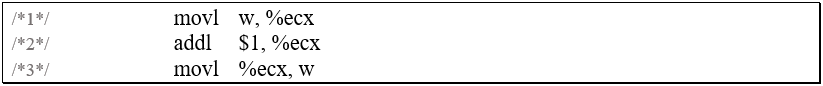
\includegraphics[width=1\linewidth]{AtomOperationExample1}
	\end{figure}
	\parЗначит, выполнять операцию инкремента некоторой переменной в нескольких потоках одновременно - небезопасно, т.к. при выполнении ассемблерной инструкции /*2*/ поток может быть прерван и процессор передан во владение другому потоку, который получит некорректное значение недоинкрементированной переменной.
	\parЛогично было бы предположить, что операции присваивания не должны обладать описанным недостатком. Действительно, в Ассемблере есть отдельная инструкция для записи значения переменной по указанному адресу. К сожалению, это предположение не до конца верно: действительно, при выполнении присваивания переменной типа char эта операция будет выполнена единой ассемблерной инструкцией. Однако с другими типами данных этого нельзя сказать наверняка. Общее практическое правило можно грубо сформулировать так: "атомарность операции присваивания гарантируется только для операций с данными, разрядность которых не превышает разрядности процессора". 
	\parНапример, при присваивании переменной типа int на 32-разрядном процессоре будет сгенерирована одна ассемблерная инструкция. Однако при компиляции этой же операции на 16-разрадном компьютере будет сгенерировано две ассемблерные команды для независимой записи младших и старших бит.
	\parСледует иметь в виду, что сформулированное правило работает при присваивании переменных и выражений, однако не всегда может выполняться при присваивании констант. Рассмотрим пример С-кода, в котором 64-разрядной переменной s (тип uint64\textunderscore t) присваивается большое число, заведомо превышающее 32-разрядную величину:
	\begin{figure}[H]
		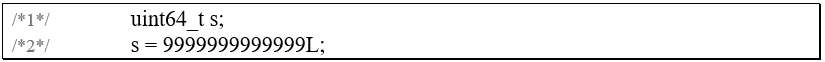
\includegraphics[width=1\linewidth]{AtomOperationExample2}
	\end{figure}
	\parЭтот код будет транслирован в следующий ассемблерный код на 64-разрядном процессоре:
	\begin{figure}[H]
		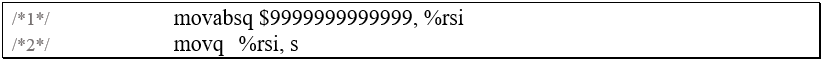
\includegraphics[width=1\linewidth]{AtomOperationExample3}
	\end{figure}
	\parКак видим, операция присваивания была транслирована в две ассемблерные инструкции, что делает невозможным безопасное распараллеливание такой операции.
	\parСформулированное правило применимо не только к операции присваивания, но и к операции чтения переменной из памяти, поэтому любую из этих операций в потокобезопасной среде придётся защищать мьютексами или критическими секциями.
	\parОсобый случай атомарного изменения данных - это изменение структуры. Для этого надо использовать CAS-операцию с указателем на эту структуру. Выполняя такую операцию, процессор создаст вторую структуру данных с заданными полями и сравнит её со старой версией структуры. Если значение хотя бы одного поля поменялось, то он атомарно подменит указатель. В этом есть накладные расходы: даже простое изменение одного поля структуры требует создание полной копии структуры, чтобы потом подменить указатель.
	\par
}